% \documentclass[12pt, twoside]{article}
\usepackage[letterpaper, margin=1in, headsep=0.2in]{geometry}
\setlength{\headheight}{0.6in}
%\usepackage[english]{babel}
\usepackage[utf8]{inputenc}
\usepackage{microtype}
\usepackage{amsmath}
\usepackage{amssymb}
%\usepackage{amsfonts}
\usepackage[nomessages]{fp} %\FPeval{\var-name}{2*sin(pi/6)}
\usepackage{siunitx} %units in math. eg 20\milli\meter
\usepackage{yhmath} % for arcs, overparenth command
\usepackage{tikz} %graphics
\usetikzlibrary{quotes, angles, arrows, arrows.meta}
\usepackage{graphicx} %consider setting \graphicspath{{images/}}
\usepackage{parskip} %no paragraph indent
\usepackage{enumitem}
\usepackage{multicol}
\usepackage{venndiagram}

\usepackage{fancyhdr}
\pagestyle{fancy}
\fancyhf{}
\renewcommand{\headrulewidth}{0pt} % disable the underline of the header
\raggedbottom
\hfuzz=2mm %suppresses overfull box warnings

\usepackage{hyperref}

\fancyhead[LE]{\thepage}
\fancyhead[RO]{\thepage \\ Name: \hspace{4cm} \,\\}
\fancyhead[LO]{BECA / Dr. Huson / Geometry\\*  Unit 3: Parallel lines and transversals\\* 28 October 2022}

\begin{document}

\subsubsection*{3.8 Test: Parallel lines, transversals, and triangle angles}
\begin{enumerate}
\item Identify the true relationships among angles made by two parallel lines and a transversal.
\begin{multicols}{2}
  \begin{enumerate}
    \item T \hspace{0.5cm} F \hspace{1cm} $\angle 1 \cong \angle 4$
    \item T \hspace{0.5cm} F \hspace{1cm} $\angle 2 \cong \angle 6$
    \item T \hspace{0.5cm} F \hspace{1cm} $m\angle 4 + m\angle 5 =  180$
    \item T \hspace{0.5cm} F \hspace{1cm} $m\angle 2 + m\angle 8 =  180$
  \end{enumerate}
    \begin{tikzpicture}[scale=1]
    \draw [<->, thick] (3,2)--(8,2);
    \draw [<->, thick] (2,0)--(7,0);
    \draw [<->, thick] (4,-1)--(5.5,3);
    \node at (4.5,0.3) [left]{$5$};
    \node at (4.5,0.3) [right]{$6$};
    \node at (4.3,-0.3) [left]{$7$};
    \node at (4.3,-0.3) [right]{$8$};
    \node at (5.2,2) [above left]{$1$};
    \node at (5.2,2) [above right]{$2$};
    \node at (5,2) [below left]{$3$};
    \node at (5,2) [below right]{$4$};
  \end{tikzpicture}
\end{multicols}

\item Find $x$ given two parallel lines and a transversal, with alternate interior angles measuring
  \begin{multicols}{2}
  $\displaystyle m\angle 3 = x$ \hspace{0.75cm}$\displaystyle m\angle 6 = 80^\circ$
  \begin{flushright}
  \begin{tikzpicture}[scale=1,rotate=-10]
    \draw [<->, thick] (3,2)--(8,2);
    \draw [<->, thick] (2,0)--(7,0);
    \draw [<->, thick] (4,-1)--(5.5,3);
    \node at (4.5,0.3) [left]{$5$};
    \node at (4.5,0.3) [right]{$6$};
    \node at (4.3,-0.3) [left]{$7$};
    \node at (4.3,-0.3) [right]{$8$};
    \node at (5.2,2) [above left]{$1$};
    \node at (5.4,2) [above right]{$2$};
    \node at (4.9,2) [below left]{$3$};
    \node at (5,2) [below right]{$4$};
  \end{tikzpicture}
  \end{flushright} 
  \end{multicols}

\item Given parallelogram with angle measure $110^\circ$, as shown. Find the measure of the opposite internal angle, $x$. \par \medskip
\begin{tikzpicture}[scale=1]
  \draw[thick] (0,0)--(110:2.13)--+(5,0)--(5,0)--cycle;
  %\node at (1.5, 0.25){m$\angle 2 = 110^\circ$};
  \node at (4.1, 1.7){$x^\circ$};
  \draw (0.4,0) arc (0:110:0.4)node[pos=0.5, right]{$110^\circ$};
\end{tikzpicture} \bigskip

\item Given two parallel lines, two transversals.
  \begin{multicols}{2}
    \begin{enumerate}
      \item Find $x$, $y$
      \item Circle the relationship depicted.
      \begin{itemize}
        \item vertical angles
        \item corresponding angles
        \item same-side exterior angles
        \item alternate interior angles
      \end{itemize}
    \end{enumerate}
      \begin{tikzpicture}[scale=1.4]
      \draw [<->, thick] (4,2.25)--(7,2.25);
      \draw [<->, thick] (3.5,0)--(7,0);
      \draw [<->, thick] (4,-0.5)--(5.7,3);
      \draw [<->, thick] (6.5,-0.5)--(5,3);
      \node at (4.4,0.3) [right]{$72^\circ$};
      \node at (5.5,0.3) [right]{$81^\circ$};
      \node at (5.1,2.2) [below left]{$x$};
      \node at (5.5,2.2) [below right]{$y$};
    \end{tikzpicture}
  \end{multicols}

\newpage
\subsubsection*{Do Not Solve}
\item Given two parallel lines and a transversal, with same-side interior angles $m\angle 3 = 7x$ and $m\angle 5 = 3x + 10$. Write an equation, to solve for $x$, but do not solve it. %Write an equation, then solve for $x$.
\begin{flushright}
  \begin{tikzpicture}[scale=1]
    \draw [<->, thick] (0,0)--(7,0);
    \draw [<->, thick] (1,2)--(8,2);
    \draw [<->, thick] (5,-1)--(3,3);
    %\draw [<->, thick] (11,-1)--(9,3);
    %\node at (4, 1.7){$1$};
    \node at (2.5, 2)[below]{$m\angle 3 = 7x$};
    \node at (4.2, 0)[above left]{$m\angle 5 = 3x + 10$};
    %\node at (10, 0.25){$3$};
  \end{tikzpicture}
  \end{flushright}

\item Two parallel lines intersect a transversal, shown. Given the corresponding angles  $m\angle 2 = 11x - 25$ and $m\angle 6 = 6x + 30$. Write an equation, but do not solve it. %Solve for $x$ then find the measure of $\angle 4$. 
  \begin{flushright}
    \begin{tikzpicture}[scale=1]
      \draw [<->, thick] (3,0)--(9,0);
      \draw [<->, thick] (2,2)--(8,2);
      \draw [<->, thick] (5,-1)--(3,3);
      %\draw [<->, thick] (11,-1)--(9,3);
      %\node at (4, 1.7){$1$};
      \node at (5.3, 2)[above]{$m\angle 2 = 11x - 25$};
      \node at (6.2, 0.25){$m\angle 6 = 6x + 30$};
      %\node at (10, 0.25){$3$};
    \end{tikzpicture}
    \end{flushright} \vspace{1cm}

\subsubsection*{For the remaining problems, write an equation, solve for $x$, and check it.}
  \item Given two parallel lines that intersect a transversal,  $\overleftrightarrow{DE} || \overleftrightarrow{BC}$. $m\angle ABC =3x-10$ and $m\angle BDE=6x+10$. Find $x$. \par \bigskip
      \begin{tikzpicture}[scale=1.1]
        \draw [<->, thick] (-1,0)--(0,0)--(4,0);
        \draw [<->, thick] (-0.5,-0.5)--(3,3)--(3.5,3.5);
        \draw [<->, thick] (1,2)--(5, 2)--(5.5,2);
        \draw [fill] (3,3) circle [radius=0.05] node[above left]{$A$};
        \draw [fill] (5, 2) circle [radius=0.05] node[below]{$E$};
        \draw [fill] (2,2) circle [radius=0.05] node[above left]{$D$};
        \draw [fill] (0,0) circle [radius=0.05] node[above left]{$B$};
        \draw [fill] (3,0) circle [radius=0.05] node[below]{$C$};
      \end{tikzpicture} \vspace{3cm}

\newpage
\item Given two vertical angles as shown, $m \angle 1 = 2x-30$, and $m \angle 2 = x+20$. Find $x$.
  \begin{flushright}
  \begin{tikzpicture}[scale=.7]
    \draw [<->, thick] (0,-1.5)--(10,1.5);
    \draw [<->, thick] (2,3.5)--(7,-3.5);
    \node at (3,.4){1};
    \node at (6,-.6){2};
    %\draw [fill] (0,0) circle [radius=0.05] node[below]{$P$};
    %\draw [fill] (6,0) circle [radius=0.05] node[below]{$R$};
    %\draw [fill] (3,0) circle [radius=0.05] node[below]{$Q$};
  \end{tikzpicture}
  \end{flushright} \vspace{1cm}

\item The ray $\overrightarrow{BD}$ is the angle bisector of $\angle ABC$. Given that the angle measures are m$\angle ABD = 6x+19$ and m$\angle CBD = 9x-11$, find $x$. \par \bigskip
  \begin{flushright}
    \begin{tikzpicture}[scale=1, rotate=10]
      \draw[<->, thick]
        (0:3) coordinate (a) node[above left] {$C$}
        -- (0,0) coordinate (b) node[below] {$B$}
        -- (80:3) coordinate (c) node[above right] {$D$}
        pic["$9x-11$", <->, draw=black, angle eccentricity=1.5, angle radius=1.5cm]
        {angle=a--b--c};
        \draw[<-, thick]
        (160:3) coordinate (d) node[above left] {$A$}
        -- (0,0) coordinate (e)
        pic["$6x+19$", <->, draw=black, angle eccentricity=1.5, angle radius=1.5cm]
        {angle=c--e--d};
    \end{tikzpicture}
  \end{flushright} \vspace{1cm}

\item Given $\overrightarrow{BA} \perp \overrightarrow{BC}$, $m \angle ABD = 2x-18$, and $m \angle DBC = 4x$. Find $x$. 
\begin{flushleft}
\begin{tikzpicture}[scale=1]
  \draw [<->, thick] (0,4)--(0,0)--(5,0);
  \draw [->, thick] (0,0)--(70:3.5);
  \draw [-, thin] (0, 0.4)--(0.4, 0.4)--(0.4, 0);
  %\node at (3,.4){1};
  %\node at (6,-.6){2};
  \draw [fill] (0,0) circle [radius=0.05] node[below]{$B$};
  \draw [fill] (0,3) circle [radius=0.05] node[left]{$A$};
  \draw [fill] (4,0) circle [radius=0.05] node[below]{$C$};
  \draw [fill] (70:2.5) circle [radius=0.05] node[below right]{$D$};
\end{tikzpicture}
\end{flushleft}
    
\newpage
\item Given isosceles $\triangle LMN$, $\overline{LM} \cong \overline{NM}$. If $m\angle L=3x$ and $m\angle N=75^\circ$, find $x$.
  \begin{flushright}
  \begin{tikzpicture}[scale=0.8]
    %\draw [->, thick] (0,0)--(5,5);
    \draw [-, thick] (0,0) node[below]{$L$}--
      (2.5,3) node[above]{$M$}--
      (5,0) node[below]{$N$}--cycle;
  \end{tikzpicture}
  \end{flushright}

\item The measures in degrees of the three angles of a triangle are $2x$, $\frac{1}{2}x$, and $80^\circ$. Find $x$. \vspace{4cm}

\item Given  $\triangle EFG$ with $\overline{EF}$ extended to $A$. If $m\angle F=38^\circ$ and $m\angle AEG=133^\circ$, find $m\angle G=x^\circ$.
  \begin{flushright}
    \begin{tikzpicture}%[scale=0.7]
      \draw [thick](0,0)node[below]{$A$}--
        (2,0)node[below]{$E$}--
        (8,0)node[below]{$F$}--
        (4,3)node[above]{$G$} --(2,0);
    \end{tikzpicture}
  \end{flushright}

\item Given parallel lines $\overleftrightarrow{AB} \parallel \overleftrightarrow{CF}$, $m\angle BAE=75^\circ$ and $m\angle DAE=55^\circ$. \\[0.5cm]
  Find $m\angle ADC = x$ and $m\angle AEF = y$.
  \begin{flushright}
  \begin{tikzpicture}[scale=1.]
    \draw [<->, thick] (0,3)--(6.5,3) node[above left]{$B$};
    \draw [<->, thick] (-1,0) node[below right]{$C$}--
      (5,0)--
      (6,0) node[below left]{$F$};
    \draw [-, thick] (1,0) node[below]{$D$}--
      (2.5,3) node[above]{$A$}--
      (4.35,0) node[below]{$E$};
    \node at (2.6,2.4)[below]{$55^\circ$};
    \node at (2.9,2.8)[below right]{$75^\circ$};
    \node at (1,0)[above left]{$x$};
    \node at (4.4,0)[above right]{$y$};
  \end{tikzpicture}
  \end{flushright}


\end{enumerate}
\end{document}